\documentclass{article}
\usepackage[utf8]{inputenc}
\textheight = 25cm 
\textwidth = 15cm
\topmargin = -2.5cm 
\oddsidemargin = 1.5cm
\usepackage{float}
\usepackage{graphicx}
\graphicspath{{./images/}}

\usepackage{amsmath}
\usepackage{mathtools, xparse}
\usepackage[shortlabels]{enumitem}
\usepackage[most]{tcolorbox}
\usepackage{adjustbox}
\usepackage{bm} 

\DeclarePairedDelimiter{\norm}{\lVert}{\rVert}

\title{Tarea 9 Mecánica Analítica}
\author{Cerritos Lira Carlos}
\date{8 de Mayo del 2020}

\begin{document}
\maketitle
\section*{Problemas}
\section*{1.-}
\subsection*{6.10)}
Una partícula positiva de carga $e$ (fig. 6-16) se mueve en el campo eléctrico central
\[ \bm{E} = -\frac{\alpha}{\rho} \bm{e}_{\rho} \]
que hay entre las placas de un condensador cilíndrico, y en un campo magnético uniforme:
\[ \bm{B} = B\bm{k} \]
paralelo al eje del condensador.
\begin{enumerate}[a)]
    \item Establecer las ecuaciones de movmiento de la partícula en coordenadas cilíndricas.
    \item Demostrar que la ecuación de movmimiento, en función de la variable anular $\phi$, que es 
    una coordenada que se puede no considerar, se resuelve fácilmente y da como integral de movmiento 
    \[ m\rho^2\dot{\phi} + \frac{1}{2}e\rho^2B = h = constante \]
    \item Demuestrar que, utilizando el resultado hallado en $b)$, la ecuación radial se puede 
    reducir a una ecuación de movimiento unidimensional, que nos dará una segunda integral del movimiento 
    que expresa la conservación de la energía total. 
    \item Si la partícula es emitida del cilindro interior con una velocidad:
    \[ \bm{v}_0 = v_0\bm{e}_p \]
    ¿cuál debe ser el valor mínimo de $v_0$ para que la partícula llegue al otro cilindro cuyo radio es $R_2$.
    [Sugerencia: el valor mínimo de $v_0$ se obtendrá cuando $R_2$ sea un punto de retorno]
\end{enumerate}
\begin{figure}[H]
    \centering
    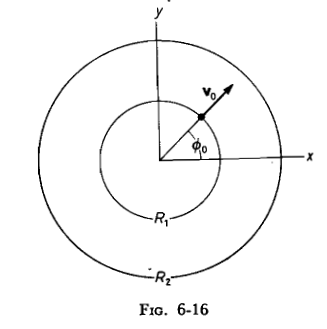
\includegraphics[scale=0.6]{images/p1_diagram.png}
\end{figure}
\begin{tcolorbox}[breakable]
    \subsubsection*{a)}
    Recordamos que en coordenadas cilíndricas:
    \begin{align*}
        \bm{r} &= \rho cos\phi \bm{i} + \rho sin\phi\bm{j} + z\bm{k} \\
        \bm{v} 
        &=(\dot{\rho} cos\phi - \rho \dot{\phi}sin\phi) \bm{i} 
        + (\dot{\rho}sin\phi + \rho \dot{\phi}cos\phi) \bm{j} 
        + \dot{z}\bm{k} \\
        \dot{r}^2 &= \dot{\rho}^2 + \rho^2\dot{\phi}^2 + z^2 \\ 
        \bm{e}_\rho &= cos\phi \bm{i} + sin\phi \bm{j} 
    \end{align*}
    El campo eléctrico y magnético son de la forma:
    \begin{align*}
        \bm{E} &= -\nabla \Phi = -\bm{\nabla} \alpha ln(\rho) \\ 
        \bm{B} &= \nabla \times \bm{A} 
    \end{align*}
    en este caso $\bm{A}$ está dado por:
    \begin{align*}
        \bm{A} 
        &= -\frac{1}{2}(\bm{r} \times \bm{B}) \\
        &= -\frac{1}{2}(\bm{r} \times B\bm{k}) \\
        &= -\frac{1}{2}B\rho(sin\phi \bm{i} - cos\phi \bm{j}) \\
        \bm{v} \cdot \bm{A} 
        &= -\frac{1}{2}B\rho 
        \bigg[ sin\phi (\dot{\rho} cos\phi - \rho \dot{\phi}sin\phi) 
        -cos\phi (\dot{\rho}sin\phi + \rho \dot{\phi}cos\phi) \bigg] \\
        &= \frac{1}{2}B\rho^2 \dot{\phi}(cos\phi^2 + sin\phi^2) \\
        &= \frac{1}{2}B\rho^2 \dot{\phi} 
    \end{align*}
    de donde obtenemos:
    \begin{align*}
        L 
        &= T - U + e\bm{v} \cdot \bm{A} \\
        &= \frac{1}{2}m(\dot{\rho}^2 + \rho^2\dot{\phi}^2 + z^2) - e\alpha ln(\rho) + \frac{1}{2}eB\rho^2 \dot{\phi}
    \end{align*}
    recordamos que se satisface la relación:
    \begin{align*}
        \frac{\partial L}{\partial q_i} - \frac{d}{dt}\frac{\partial L}{\partial \dot{q}_i} &= 0
    \end{align*}
    aplicado a $\phi$ obtenemos:
    \begin{align*}
        \frac{\partial L}{\partial \phi} - \frac{d}{dt}\frac{\partial L}{\partial \dot{\phi}} &= 0 \\
        \frac{d}{dt}(m\rho^2\dot{\phi} + \frac{1}{2}eB\rho^2) &= 0
     \end{align*}
     aplicado a $\rho$ obtenemos:
    \begin{align*}
        \frac{\partial L}{\partial \rho} - \frac{d}{dt}\frac{\partial L}{\partial \dot{\rho}} &= 0 \\
        m\rho \dot{\phi}^2 - e\alpha \frac{1}{\rho} + eB\rho \dot{\phi} - \frac{d}{dt}(m\dot{\rho}) &= 0 \\
        m\rho \dot{\phi}^2 - e\alpha \frac{1}{\rho} + eB\rho \dot{\phi} - m\ddot{\rho} &= 0 
    \end{align*}
    \subsubsection*{b)}
    De la ecuación de movmiento obtenida en $a)$, para $\phi$ se tiene:
    \[ \frac{d}{dt}(m\rho^2\dot{\phi} + \frac{1}{2}eB\rho^2) = 0 \]
    de donde se obtiene la relación deseada.
    \subsubsection*{c)}
    De la ecuación de movimiento obtenida en $a)$, para $\rho$ se tiene:
    \[m\rho \dot{\phi}^2 - e\alpha \frac{1}{r} + eB\rho \dot{\phi} - m\ddot{\rho} = 0 \]
    remplazando $\dot{\phi}$ de la parte $b)$ obtenemos:
    \[ \dot{\phi} = \frac{1}{m^2}\left( \frac{h}{\rho^2} - \frac{1}{2}eB \right) \]
    remplazando obtenemos:
    \begin{align*}
        m\rho \dot{\phi}^2 - e\alpha \frac{1}{r} + eB\rho \dot{\phi} - m\ddot{\rho} &= 0 \\
        m\rho \frac{1}{m^2}\left( \frac{h}{\rho^2} - \frac{1}{2}eB \right)^2 
        - e\alpha \frac{1}{\rho} 
        + eB\rho\frac{1}{m^2}\left( \frac{h}{\rho^2} - \frac{1}{2}eB \right) - m\ddot{\rho} &= 0
    \end{align*}
    donde se observa obtuvimos una ecuación unidimensional para $\rho$
    \subsubsection*{d)}
    Sabemos que para este sistema $H=T+U$ es una constante, esto se puede comprobar si calculamos $H = p_i\dot{q}_i - L$,
     como $R_2$ es un punto de retorno $T(R_2)=0$, de donde obtenemos:
    \begin{align*}
        T(R_1) + U(R_1) &= U(R_2) \\
        \frac{1}{2}v_0^2 + \alpha ln(R_1) &= \alpha ln(R_2) \\
        v_0^2 &= 2\alpha ln\left(\frac{R_2}{R_1}\right)
    \end{align*}

\end{tcolorbox}

\section*{2.-}  
\subsection*{8.1)}
Una partícula estacionaria de masa $3m kg$, estalla en tres piezas iguales dos de las cuales
vuelan en direcciones perpendiculares entre sí, una con una velocidad $2a \frac{m}{s}$ y la
otra a $3a\frac{m}{s}$. ¿Cuál es la magnitud, dirección y sentido de la cantidad de movimiento 
del tercer fragmento?. La explosión tiene lugar en $10^{-5}s$. Hállese la fuerza que actúa sobre 
cada pieza durante la explosión.
\begin{tcolorbox}[breakable]
    Elegimos un sistema de referencia donde las partículas salgan en direcciones $\bm{i},\bm{j}$ respectivamente. \\
    Usando conservación del momento para un sistema de partículas cuando $\bm{F}^{ext} = 0$, tenemos:
    \begin{align*}
        \bm{p}_1 + \bm{p}_2 + \bm{p}_3 &= 0 \\
        2ma \bm{i} + 3ma \bm{j} + \bm{p}_3 &= 0 \\
        \bm{p}_3 &= -m(2a\bm{i} + 3a \bm{j})
    \end{align*}
    Obtenemos la fuerza usando la relación:
    \begin{align*}
        \bm{p}_i(t_2) - \bm{p}_i(t_1) &= \int_{t_1}^{t_2} F_i(t)dt \\
        \bm{p}_i &= F_i(t_2-t_1) \\
        F_i &= p_i \cdot \times 10^5 \tfrac{m}{s^2}
    \end{align*}
\end{tcolorbox}

\section*{3.-}
\subsection*{8.2)}
Un núcleo, originalmente en reposo, se desintegra por la emisión de un electrón, cuya 
cantidad de movimiento es $1.73 \frac{Mev}{C}$ y, perpendicularmente a la dirección del
electrón, de un neutrino cuya cantidad de movimiento es $1.0\frac{Mev}{c}$. ¿En qué dirección y 
sentido recaulará el núcleo?. ¿Cuál será su cantidad de movimiento en $\frac{Mev}{c}$. 
Si la masa del núcleo restante es $3.90 \times 10^{-22}g$. Si la masa del núcleo restante es 
$3.9 \times 10^{-22}g$, ¿cuál será su energía cinética en electrón volts? 
\begin{tcolorbox}[breakable]
    Usamos nuevamente la conservación del momento para un sistema de partículas donde $\bm{F}^{ext} = 0$, donde tenemos:
    \begin{align*}
        \bm{p}_1 + \bm{p}_2 + \bm{p}_3 &= 0 \\
        p_1\bm{i} + p_2\bm{j} + \bm{p}_3 &= 0 \\
        \bm{p}_3 &= -(p_1\bm{i} + p_2\bm{j})
    \end{align*}
    por lo tanto:
    \[ p_3^2 = p_1^2 + p_2^2 \]
    \[ T = \frac{1}{2}mv^2 = \frac{1}{2m}p_3^2 \]
\end{tcolorbox}

\section*{4.-}
\subsection*{8.4)}
Una partícula de masa $M_1$ y velocidad $V_1$ es capturada por un núcleo en reposo,
y otra partícula ligera de masa $M_2$ es expelida con una velocidad $V_2$ en ángulo 
recto con la trayectoria de la primera, reculando el resto del núcleo (de masa $M_3$)
con una velocidad $V_3$. Demuestre que la energía cinética de $M_2$ es:
\[ T = \frac{M_3}{M_2+M_1} \left( Q + \frac{M_3-M_1}{M_3}T_1 \right) \]
\begin{tcolorbox}[breakable]
\end{tcolorbox}

\section*{5.-}
\subsection*{8.16)}
Analícese el movimiento del regulador del problema $8.15$, si la velocidad angular 
del eje no está restringida a $w$, sino que gira libremente sin que tenga ningún momento 
rotacional externo (o par resistente) aplicando. 
\begin{enumerate}[a)]
    \item Hállese la velocidad angular de rotación estacionara para una altura dada, $z$, 
    del manguito inferior.
    \item Hállese la frecuencia de las pequeñas vibraciones por encima y por debajo de este movimiento 
    estacionario. 
    \item ¿Cuáles son las diferencias entre este movimiento y el del problema $8.15$?
\end{enumerate}
\begin{tcolorbox}[breakable]
    \subsubsection*{a)}
    \subsubsection*{b)}
    \subsubsection*{c)}
\end{tcolorbox}

\end{document}